%!TEX TS-program = xelatex
%!TEX encoding = UTF-8 Unicode

%%%%%%%%%%%%%%%%%%%%%%%%%%%%%%%%%%%%%%%%%%%%%%%%%%%%%%%%%%%%
% 改自研究生院提供的博士学位论文Latex单页模板,https://gs.bjtu.edu.cn/cms/item/477.html
% !!!第二章和第三章已总结了笔者撰写论文过程中使用的技巧及遇到的问题解决方案,建议论文撰写者仔细阅读。

% 支持的学位类型:博士、学硕
% 支持的页面格式:单面、双面
% 单面格式:边距居中,便于PDF阅读,论文撰写、匿名送审、在线送审时用此格式。注意,学校要求,页数少于一定数量时则需要用此格式打印纸质版。
% 双面格式:双面打印模式,在这种模式下奇偶页左侧边距不同,会自动生成空白页,确保新章节从奇数页码开始。
% 博士学位论文主体部分字数一般为6~10万字(含图表);硕士学位论文主体部分字数一般为3~5万字(含图表)。

% 使用说明:
% 1. 纸质版及图书馆最终提交电子版请在demo.tex中使用twoside
% 2. 匿名送审和在线送审的电子版,去掉twoside就是单页模板,便于电子阅读。
% 3. 理论上硕士与博士模板通用,修改demo.tex中\documentclass命令即可,硕士使用建议再核对一下格式。
% 4. 编译环境:在线可以用overleaf,即www.overleaf.com;离线可以用TexLive+TexStudio
% 5. 编译请使用xelatex

% 修改/完善的内容包括:
% 1. 与最新word模板同步,添加了答辩名单页、答辩决议页
% 2. 修正twoside中的偶数空白页页眉页脚问题,见demo.tex
% 3. 修正页脚字体大小及间距
% 4. 修改英文和数字字体为Times New Roman
% 5. 设置图表描述默认为居中对齐
% 6. 修正itemize的行距与正文一致
% 7. 增添命令来打中文括弧,避免正文中直接写中文括号出现的文字光标错位问题
%
% by 赵苡积,2023.05
%%%%%%%%%%%%%%%%%%%%%%%%%%%%%%%%%%%%%%%%%%%%%%%%%%%%%%%%%%%%

%\documentclass[Doctor,UTF-8]{BJTU-thesis}            %%博士,单面
\documentclass[Doctor,UTF-8,twoside]{BJTU-thesis}     %%博士,双面
%\documentclass[AcMaster]{BJTU-thesis}                %%学硕,单面
%\documentclass[AcMaster,UTF-8,twoside]{BJTU-thesis}  %%学硕,双面


%% 指定图片路径
\graphicspath{{./figures/}}

%% 添加需要的包

%清除twoside中偶数空白页的页眉页脚
\usepackage{emptypage} 

%用命令来打中文括弧,避免正文中直接写中文括号出现的文字光标错位问题
\newcommand{\cp}[1]{(#1)} %全括弧,\cp{1} -> (1)
\newcommand{\rp}[1]{#1)}   %右括弧,\rp{1} ->  1)
\newcommand{\refeq}[1]{(\ref{#1})} %自定义指令,正文引用公式时的括弧为中文括弧,如公式\refeq{eq:xxx}所示 -> 如公式(2.1)所示

%公式修正
\usepackage[T1]{fontenc}  %搭配mathptmx
\usepackage{mathptmx}     %修正部分公式中字体样式,如避免\hat的帽子间距错误,mathptmx在win和mac系统中兼容性均较好
\usepackage[mathcal]{euscript} %花体,用scr代替cal

%分块矩阵
\usepackage{blkarray}

%三线表
\usepackage{booktabs} 
\usepackage{makecell} %合并单元格
\usepackage{threeparttable} %三线表,加表格脚注
\usepackage[figuresright]{rotating} %图表旋转,超大图表需要用\begin{sidewaysfigure}和\begin{sidewaystable}旋转

%图表标题居中对齐
\usepackage[justification=centering]{caption}

%中文样式的算法表格
\usepackage[ruled]{algorithm2e}  
\renewcommand{\algorithmcfname}{算法}  %算法表头,algorithm->算法
\SetKwInput{KwIn}{输入}   % input  -> 输入
\SetKwInput{KwOut}{输出}  % output -> 输出
\SetAlgoCaptionSeparator{ :} %表头冒号变成中文冒号

% 公式符号加粗
\newcommand{\mat}[1]{{\bf #1}}           %定义矩阵符号命令,\mat{X}
\newcommand{\tensor}[1]{{\mathcal #1}}   %定义张量符号命令,\mat{X}
\renewcommand{\vec}[1]{{\boldsymbol #1}} %定义向量符号命令,\mat{x}

% 临时补充一个定理定制:
\newtheoremstyle{mythm}
{} % <上方间距>若留空,则使用默认值
{} % <下方间距>若留空,则使用默认值
{} % <主体字体>如 \itshape
{\parindent} % <缩进长度>若留空,则无缩进;可以使用 \parindent 进行正常段落缩进
{\bfseries}  % <定理头字体>如 \bfseries
{:} %<定理头后的标点符号> 如点号、冒号
{ }  %<定理头后的间距> 不可留空,若设置为 { },则表示正常词间间距;若设置为 {\newline},则环境内容开启新行
{}   %<定理头格式指定> 一般留空

\theoremstyle{mythm} % 声明定理的风格
\newtheorem{Definition}{定义}[chapter]
\newtheorem{Theorem}{定理}[chapter]
\newtheorem{Lemma}{引理}[chapter]
\newtheorem{Proof}{证明}[chapter]
\renewcommand*{\qedsymbol}{[证毕]} % 把证明的结尾改成证毕




%%%%%%%%%%%%%%%%%填写封面信息%%%%%%%%%%%%%%%%%%%%%%%%
\author{xxx}                                %作者姓名
\studentNumber{xxx}                         %学号
\advisor{xxx}                               %导师姓名
\advisorTitle{教授}                         %导师职称
\degreeType{工学}                           %学位类型
\major{计算机科学与技术}                     %专业
\researchArea{数据与知识工程}                %研究方向
\title{论文题目}                            %论文题目
\englishtitle{The Title in English.}       %英文题目
\datetime{xx年xx月}
%%%%%%%%%%%%%%%%%%%%%%%%%%%%%%%%%%%%%%%%%%%%%%

\begin{document}
	\makecover                                                  %封面
	\chapter*{学位论文版权使用授权书}
\thispagestyle{empty}


本学位论文作者完全了解北京交通大学有关保留、使用学位论文的规定。特授权北京交通大学可以将学位论文的全部或部分内容编入有关数据库进行检索,提供阅览服务,并采用影印、缩印或扫描等复制手段保存、汇编以供查阅和借阅。同意学校向国家有关部门或机构送交论文的复印件和磁盘。学校可以为存在馆际合作关系的兄弟高校用户提供文献传递服务和交换服务。

(保密的学位论文在解密后适用本授权说明)


\vspace{72pt}
学位论文作者签名:\hspace{0.2em}
\includegraphics[height=2\baselineskip]{signature.png}\hspace{2em}导师签名:\hspace{0.1em}
\includegraphics[height=2\baselineskip]{signature.png}


\vspace{12pt}
签字日期:xx年xx月xx日\hspace{7em}签字日期:xx年xx月xx日



 								%版权声明
	\twosideEmptyPage                                           %版权声明背面的空白页,只在双面时生效
	\makeInfo                                                   %内封页
	%!TEX TS-program = xelatex
%!TEX encoding = UTF-8 Unicode

\begin{committee}\zihao{-4}
\renewcommand\arraystretch{2}

\begin{table}[!h]
\centering
\begin{tabular}{|p{2.6cm}<{\centering}|p{3cm}<{\centering}|p{5cm}<{\centering}|p{2.5cm}<{\centering}|}
\hline
\textbf{答辩委员会} & \textbf{姓名} & \textbf{工作单位} & \textbf{职称} \\
\hline
主席 &   &   &   \\
\hline
委员 &   &   &   \\
\hline
委员 &   &   &   \\
\hline
委员 &   &   &   \\
\hline
委员 &   &   &   \\
\hline
秘书 &   &   &   \\
\hline
\end{tabular}	
\end{table}
\end{committee} 								%答辩委员会名单
	\setlength{\baselineskip}{20pt}
\begin{thanks}
	
放置在摘要页前,对象包括:1)国家科学基金,资助研究工作的奖学金基金,合同单位,资助或支持的企业、组织或个人。2)协助完成研究工作和提供便利条件的组织或个人。3)在研究工作中提出建议和提供帮助的人。4)给予转载和引用权的资料、图片、文献、研究思想和设想的所有者。5)其他应感谢的组织和个人。


\end{thanks} 									%致谢
	\setlength{\baselineskip}{20pt}
\begin{abstract}


\textbf{第二章和第三章已总结了笔者撰写论文过程中使用的技巧及遇到的问题解决方案,建议论文撰写者仔细阅读。}

[鼠标左键单击选择该段落,输入替换之。内容为小四号宋体。] 中文摘要应将学位论文的内容要点简短明了地表达出来,硕士学位论文一般为500-1000字,博士学位论文一般为1000-2000字。留学生英文版学位论文不少于3000字中文摘要,留学生英文版博士学位论文不少于5000字中文摘要。字体为宋体小四号。内容应包括工作目的、研究方法、成果和结论。要突出本论文的创新点,语言力求精炼。为了便于文献检索,应在本页下方另起一行注明论文的关键词(3-8个),如有可能,尽量采用《汉语主题词表》等词表提供的规范词。图X幅,表X个,参考文献X篇。


	\noindent\keywords{xxx;xxx;xxx}
\end{abstract}   								%中文摘要
	 \setlength{\baselineskip}{20pt}
\begin{englishabstract}

	English Abstract.English Abstract.English Abstract.English Abstract.English Abstract.English Abstract.English Abstract.English Abstract.English Abstract.English Abstract.English Abstract.English Abstract.English Abstract.English Abstract.English Abstract.English Abstract.English Abstract.English Abstract.English Abstract.English Abstract.English Abstract.

	\noindent\englishkeywords{xxx; xxx; xxx}
\end{englishabstract}  					    %英文摘要
%	 \setlength{\baselineskip}{20pt}
\begin{preface}
	[鼠标左键单击选择该段落,输入替换之。内容为小四号宋体。] 学位论文的序或前言,一般是作者或他人对本篇论文基本特征的简介,如说明研究工作缘起、背景、主旨、目的、意义、编写体例,以及资助、支持、协作经过等;也可以评述和对相关问题发表意见。这些内容也可以在正文引言中说明。
		
	
\end{preface}                                  %序言


	\tableofcontents                                            % 目录
    	\newpage\pagenumbering{arabic}                              %页码切回阿拉伯数字

    	%正文
    	\setlength{\baselineskip}{20pt}
\chapter{引言}
\label{cha:intro}

\textbf{第二章和第三章已总结了笔者撰写论文过程中使用的技巧及遇到的问题解决方案,建议论文撰写者仔细阅读。}

[鼠标左键单击选择该段落,输入替换之。内容为小四号宋体。] 引言(或绪论)简要说明研究工作的目的、范围、相关领域的前人工作和知识空白、理论基础和分析、研究设想、研究方法和实验设计、预期结果和意义等。应言简意赅,不要与摘要雷同,不要成为摘要的注释。一般教科书中有的知识,在引言中不必赘述。


学位论文为了需要反映出作者确已掌握了坚实的基础理论和系统的专门知识,具有开阔的科学视野,对研究方案作了充分论证,因此,有关历史回顾和前人工作的综合评述,以及理论分析等,可以单独成章,用足够的文字叙述。正文是学位论文的核心部分,占主要篇幅,可以包括:调查对象、实验和观测方法、仪器设备、材料原料、实验和观测结果、计算方法和编程原理、数据资料、经过加工整理的图表、形成的论点和导出的结论等。


由于研究工作涉及的学科、选题、研究方法、工作进程、结果表达方式等有很大的差异,对正文内容不能作统一的规定。但是,必须实事求是,客观真切,准确完备,合乎逻辑,层次分明,简练可读。


\textbf{《北京交通大学学位论文撰写规范》:https://gs.bjtu.edu.cn/cms/item/477.html}


\section{2级标题}

命令:\textbackslash section\{2级标题\}


\subsection{3级标题}

命令:\textbackslash subsection\{3级标题\} 								%引言
	 \setlength{\baselineskip}{20pt}
\chapter{常用的命令样例}
\label{cha:chap2}

论文撰写规范参照《北京交通大学学位论文撰写规范》,以下简称《规范》。下面整理了论文撰写过程中常用的一些命令样例,以便论文撰写者查阅使用。
《北京交通大学学位论文撰写规范》见https://gs.bjtu.edu.cn/cms/item/477.html

\section{中文\cp{全角}括弧}
为了避免正文中直接写中文括弧出现的文字光标错位问题,本模板制定了两种中文括弧的命令,建议在正文中使用命令来实现中文括弧:

\textbf{半括弧},\textbackslash rp\{1\}:\rp{1}xxx。\rp{2}xxx。

\textbf{全括弧},\textbackslash cp\{1\}:\cp{1}xxx。\cp{2}xxx。

\section{公式}

公式规范参照《规范》中3.10.12节。本模板定义了一些常用的命令,包括向量、矩阵、张量、引用公式命令。下面展示一些样例,便于论文撰写者使用:

\textbf{向量},\textbackslash vec\{x\}:$\vec{x}$

\textbf{矩阵},\textbackslash mat\{x\}:$\mat{X}$

\textbf{张量},\textbackslash tensor\{x\}:$\tensor{X}$

\textbf{引用公式},引用公式时需要带有全角括号,可使用本模板定义的\textbackslash refeq命令,自带全角括号,例子:如公式\refeq{eq:ch2-split}所示。

\textbf{较长的上下标},应使用非斜体\textbackslash mathrm\{xxx\},如:$\vec{x}_{\mathrm{example}}^{\mathrm{example}}$。


%\begin{equation}\label{eq:ch2-example}
%	\vec{x}_{\mathrm{example}}^{\mathrm{example}}
%\end{equation}

\textbf{嵌入在文本中的公式},使用\$\$命令,例子:$a + b = c$。

\textbf{单独为行的公式},使用\textbackslash begin\{equation\}和\textbackslash end\{equation\}命令,较长的公式需要转行时,应尽可能在“$ = $”处回行,或者在“$ + $”、“$-$”“$*$”等记号处回行。例子:如公式\refeq{eq:ch2-split}、公式\refeq{eq:ch2-aligned}和公式\refeq{eq:ch2-align}所示。

\begin{equation}\label{eq:ch2-aligned}
	\begin{aligned}
		\dot{\hat{A}}^\dag
		&=\lambda_1\left(\tanh(k_3e_v)e_v-\sigma_1\hat{A}^\dag\right)\\
		&=\lambda_1\tanh(k_3e_v)e_v-\lambda_1\sigma_1\hat{A}^\dag
	\end{aligned}
\end{equation}

\begin{equation}\label{eq:ch2-split}
	\left\{
	\begin{split}
		\frac{\texttt{d}p(t)}{\texttt{d}t}&=v(t)\\
		\frac{\texttt{d}v(t)}{\texttt{d}t}&=u(t)-a(t)-b(t)v(t)-c(t)v^2(t)-f_2^*(\cdot)
	\end{split}
	\right.
\end{equation}




\begin{subequations}\label{eq:ch2-align}
	\begin{align}
		\dot{\hat{A}}^\dag&=\lambda_1\left(\tanh(k_3e_v)e_v-\sigma_1\hat{A}^\dag\right)\\
		\dot{\hat{b}}^\dag&=\lambda_2\left(|v||e_v|-\sigma_2\hat{b}^\dag\right)\\
		\dot{\hat{c}}^\dag&=\lambda_3\left(v^2|e_v|-\sigma_3\hat{c}^\dag\right)
	\end{align}
\end{subequations}

%
%\section{图片}
%
%图片规范参照《规范》中3.10.4节,图题采用中英文对照,中文在上,居中书写,英文\cp{Times New Roman}字体五号,中文宋体五号。
%
%图中文字用宋体(中文)或Times New Roman字体(英文),字号尽量采用5号字(当字数较多时可用小5号字,以清晰表达为原则,但在一个插图内字号要统一)。同一图内使用文字应统一。图表中物理量、符号用斜体。
%
%插图之前,文中必须有关于本插图的提示,如“见图1-1”、“如图1-1所示”等。插图与其图题为一个整体,不得拆开排写于两页。插图处的该页空白不够排写该图整体时,则可将其后文字部分提前排写,将图移到次页。有分图时,分图过多在一页内安排不下时,可转到下页,总图题只出现在下页。
%
%\textbf{单图},如图\ref{fig:ch2-f1}所示。
%
%\textbf{多图并列},如图\ref{fig:ch2-f2}所示。
%
%\textbf{巨型图},为了美观,超大规模的图可尝试旋转独占一页,本模板已添加旋转包,只需将\textbackslash begin\{figure\}和\textbackslash end\{figure\}命令中的figure换为sidewaysfigure即可。
%
%\begin{figure}[!htb]
%	\centering
%	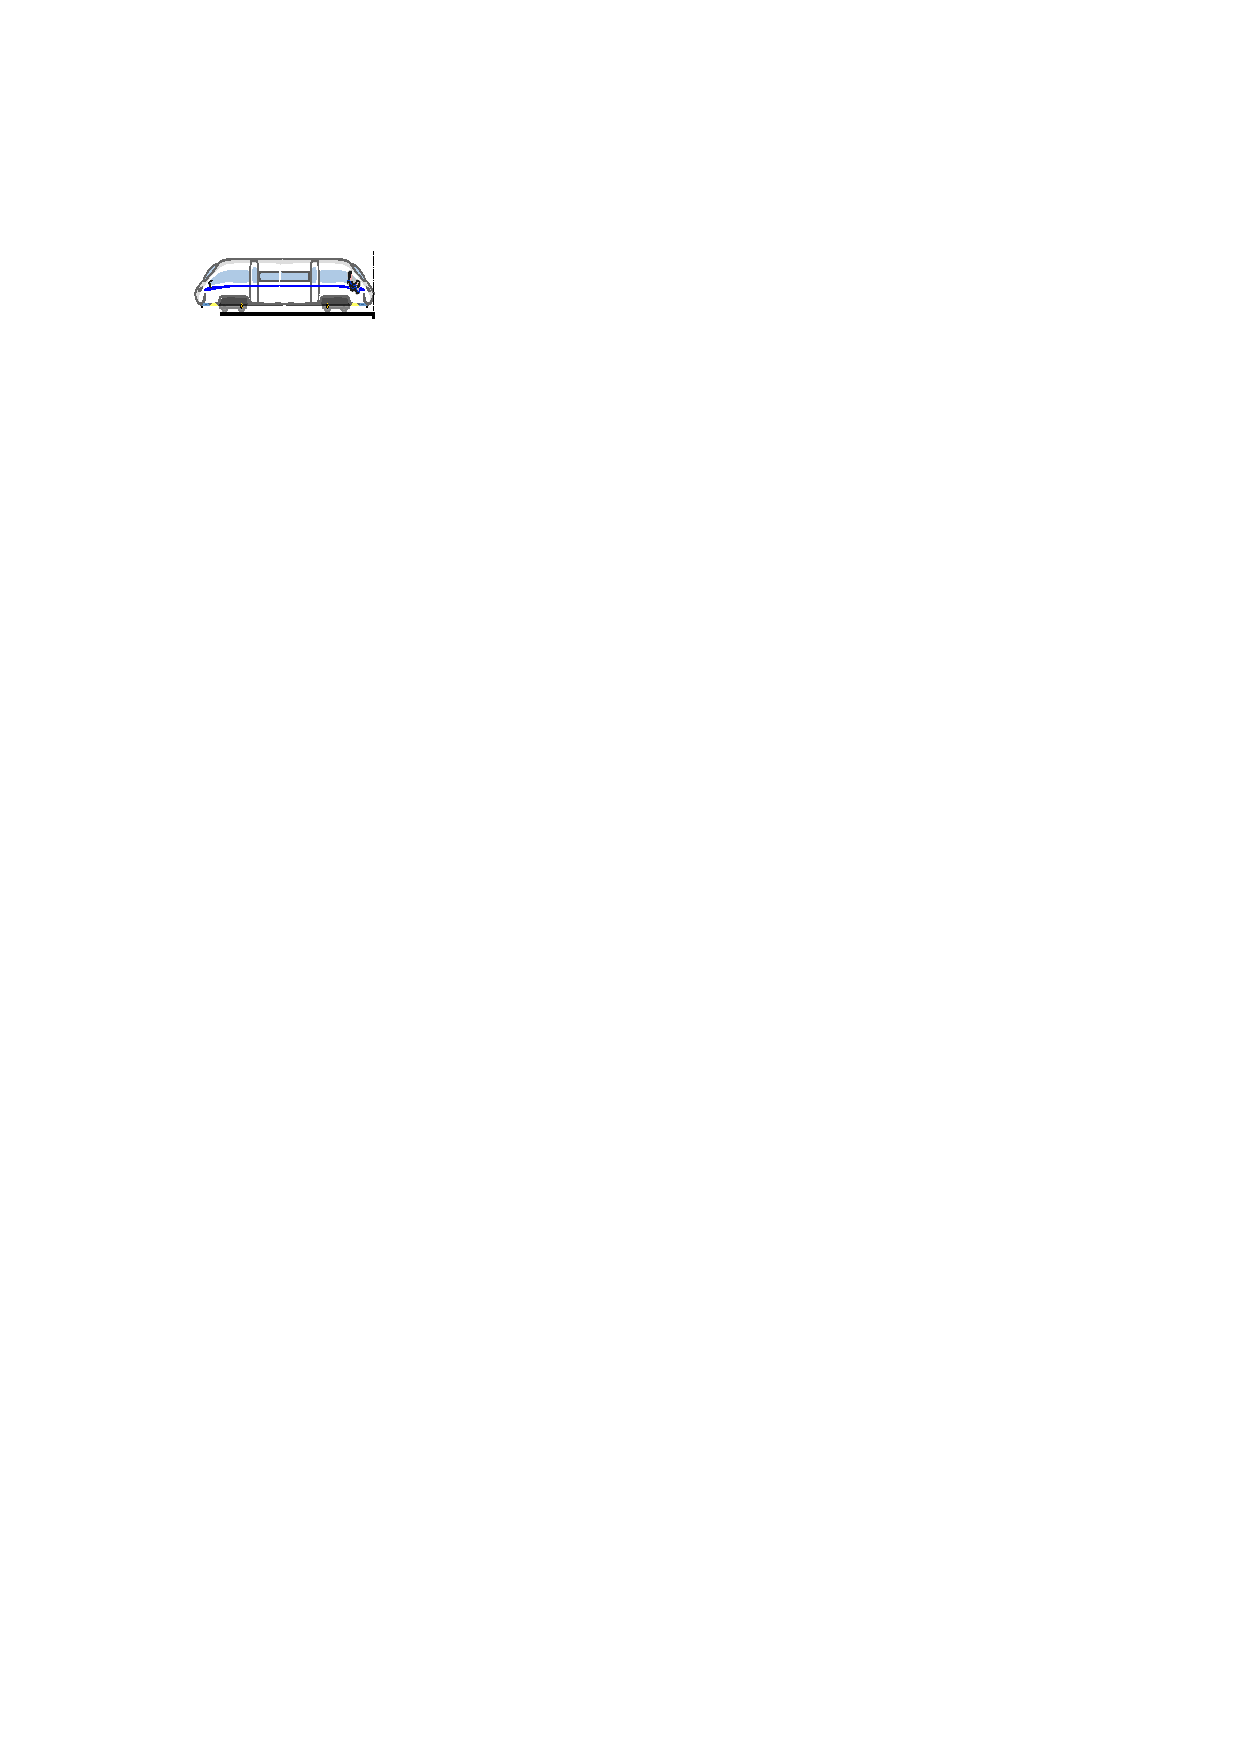
\includegraphics[scale=0.95]{figures/ch2/figure1.pdf}
%	\caption{xxx示意图。 \\Fig~\ref{fig:ch2-f1}~Illustration of xxx.}
%	\label{fig:ch2-f1}
%\end{figure}
%
%\begin{figure}[!htb]
%	\centering
%	\setlength{\belowcaptionskip}{-0.2cm} %调整图片caption与正文之间的间距,table用\abovecaptionskip。可自己调整。
%	\addtocounter{subfigure}{-1}\subfigure[Subfig1.] {\subfigure[子图1] {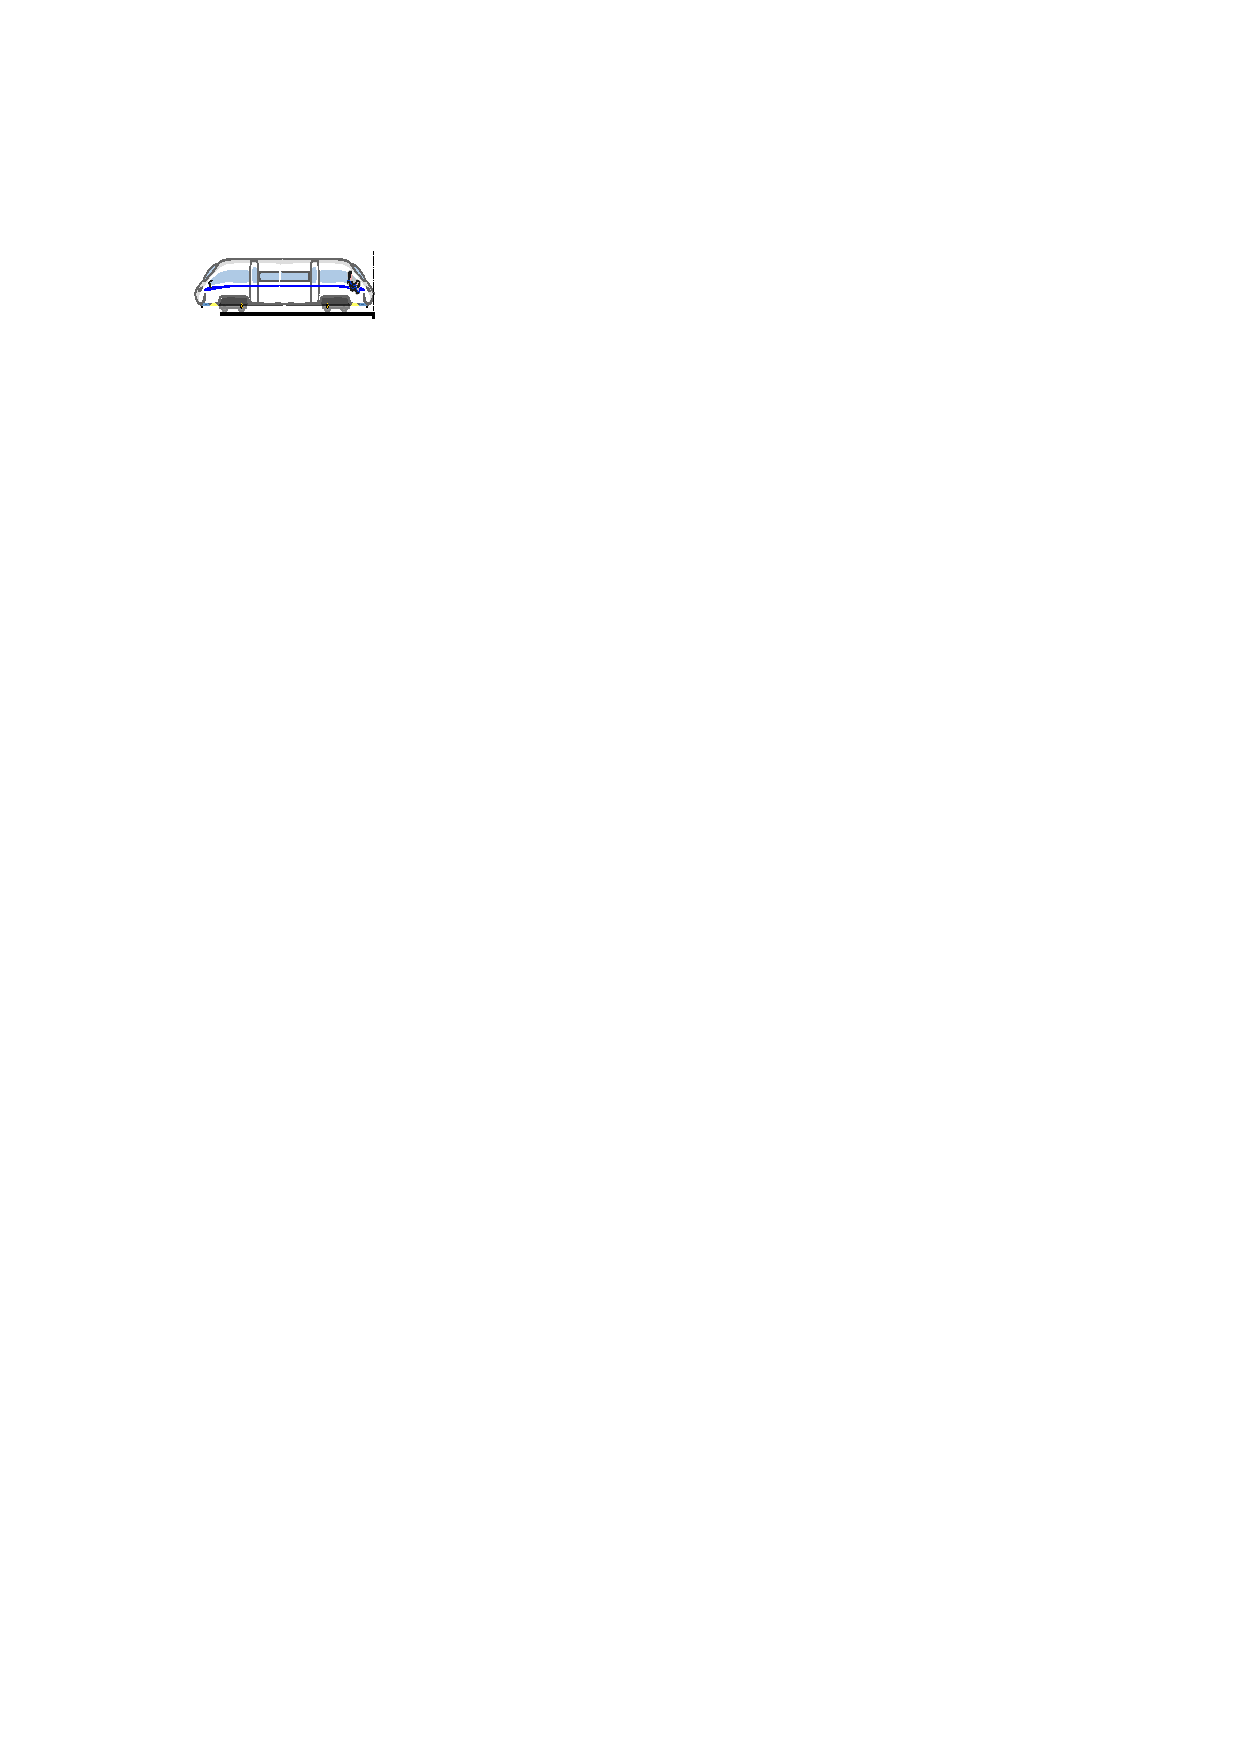
\includegraphics[scale=1]{figures/ch2/figure1.pdf}}}
%	\hspace{20pt} %子图间距
%	\addtocounter{subfigure}{-1}\subfigure[Subfig2.] {\subfigure[子图2]{ 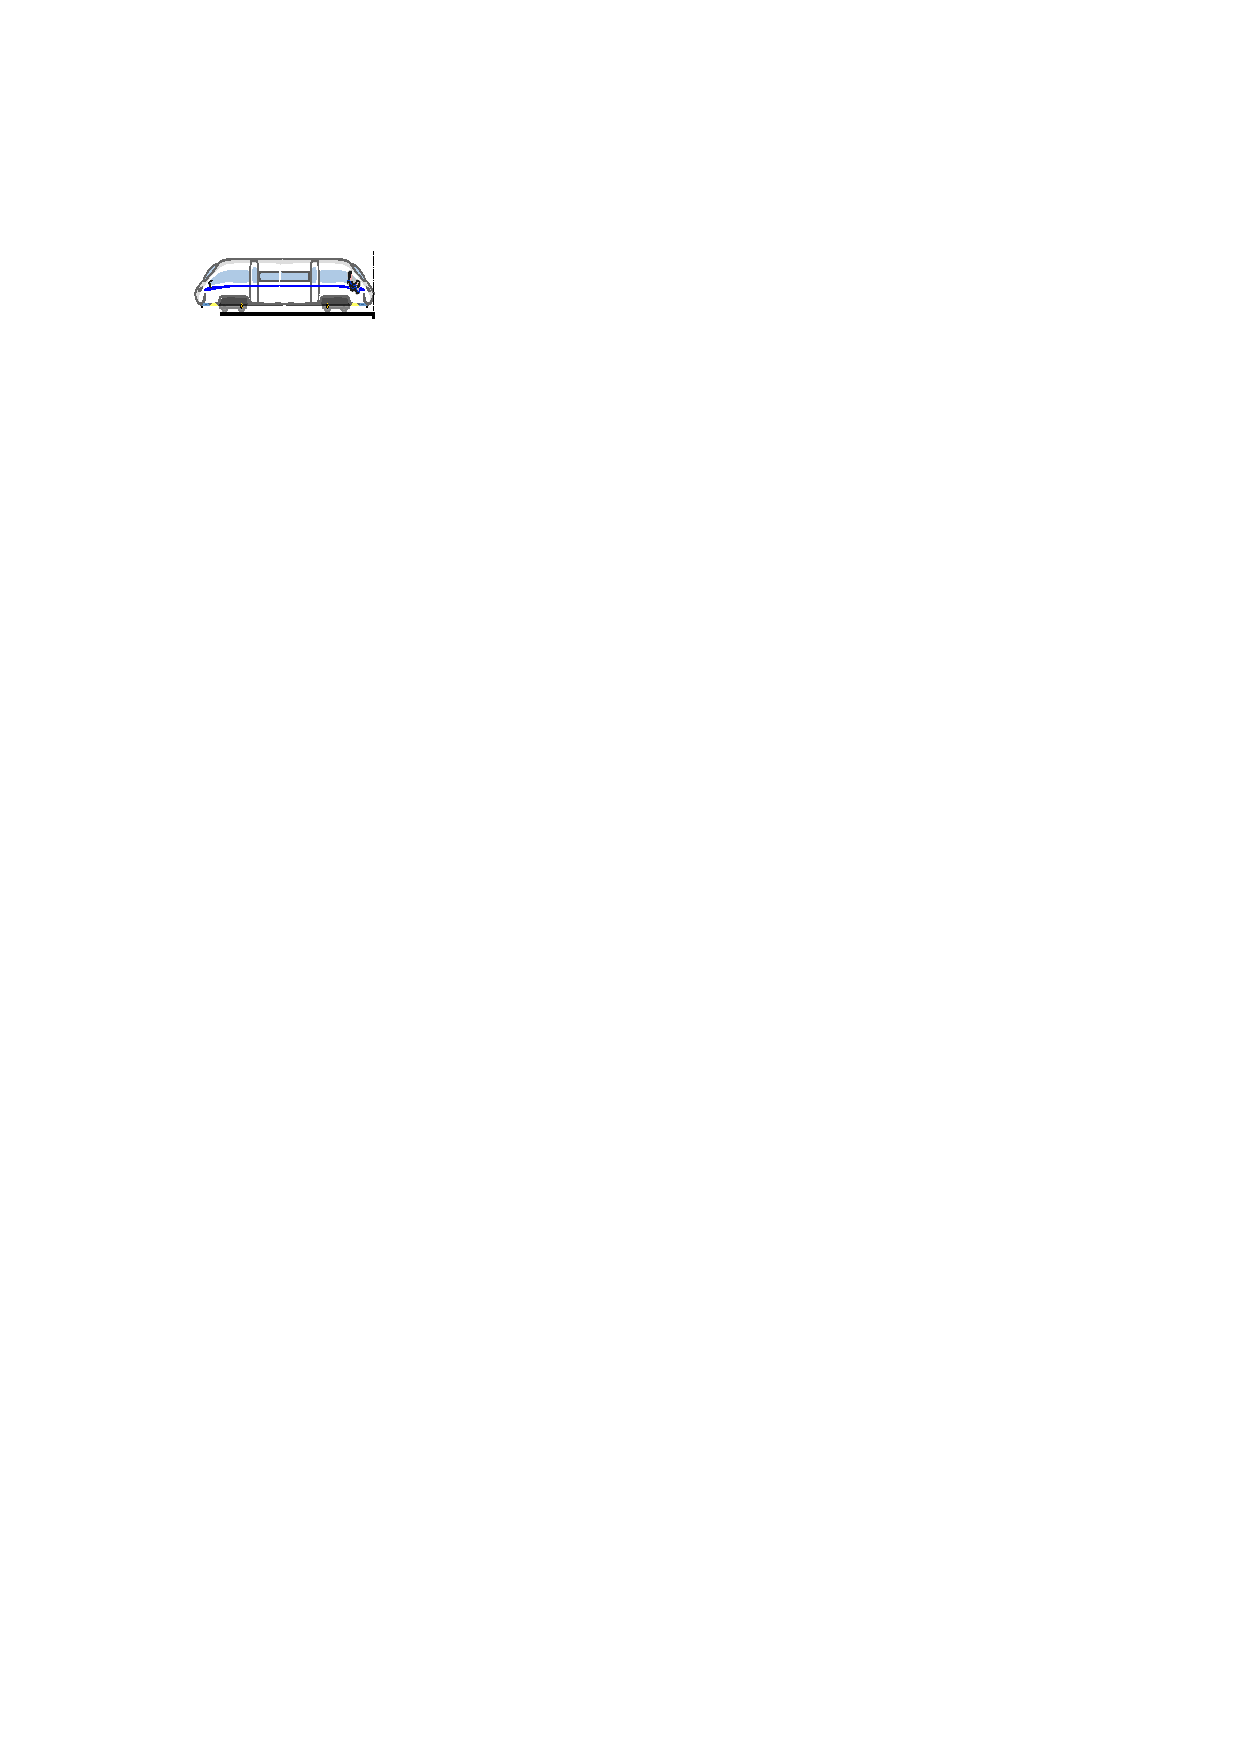
\includegraphics[scale=1]{figures/ch2/figure1.pdf}}}
%	\caption{xxx示意图。\\Fig~\ref{fig:ch2-f2}~Illustration of xxx.}
%	\label{fig:ch2-f2}
%\end{figure} 

\section{定理}


\begin{Definition}
	这是一个定义。
\end{Definition}

\begin{Theorem}
	这是一个引理。
\end{Theorem}

\begin{Proof}
	这是一个证明。
	\qed
\end{Proof}

\section{表格}

表格规范参照《规范》中3.10.5节。表题采用中英文对照,置于表的上方,居中,中文在上。英文(Times New Roman)字体五号,中文宋体五号。 

表格的编排建议采用国际通行的三线表,不加左、右边框线。表中文字用宋体(中文)或Times New Roman字体(英文),字号尽量采用5号字(当字数较多时可用小5号字,同一个插表内字号要统一)。

\textbf{普通的三线表}:如表\ref{tab:ch2_res1}所示。如果表格超出页面边距或内容太过拥挤,可以使用\textbackslash tabcolsep命令来调节列间距。

\textbf{带脚注的三线表}:如表\ref{tab:ch2_res2}所示,标题中写不下的内容可放至脚注,此时使用threeparttable包来实现。

\textbf{巨型表格}:表格过大且无法拆分成多个表格时,可以使用sidewaystable旋转表格独占一页,本模板已添加旋转包,只需将\textbackslash begin\{table\}和\textbackslash end\{table\}命令中的table换为sidewaystable即可。如表\ref{tab:ch2_res3}所示。

%\begin{table}[!htb]
%	\small %字体大小
%	%\setlength\tabcolsep{3.3pt} %调整列间距
%	\caption{性能对比。\\Table~\ref{tab:ch2_res1}~Performance comparison. }
%	\begin{tabular}{c|ccc|ccc}
%		\toprule
%		\multirow{2}{*}{模型} &  & 数据集1 &  &  & 数据集2&  \\
%		& MAE & RMSE & MAPE(\%) & MAE & RMSE & MAPE(\%) \\
%		\midrule
%		
%		SVR & 46.46 & 92.97 & 83.40 & 11.10 & 19.84 & 91.96  \\
%		LSTM & 36.20 $\pm$0.17 & 66.26 $\pm$0.80 & 40.42 $\pm$0.86 & 6.70 $\pm$0.02 & 11.36 $\pm$0.04 & 74.01 $\pm$1.26  \\
%		\bottomrule
%	\end{tabular}
%	\label{tab:ch2_res1}
%\end{table}

\begin{table}[!htb]
	\centering
	\small %字体大小
	\setlength\tabcolsep{10pt} %调整列间距
	\caption{性能对比。\\Table~\ref{tab:ch2_res1}~Performance comparison. }
	\begin{tabular}{c|ccc}
		\toprule
		模型 & MAE & RMSE & MAPE(\%)  \\
		\midrule
		LSTM & 36.20 $\pm$0.17 & 66.26 $\pm$0.80 & 40.42 $\pm$0.86 \\
		\bottomrule
	\end{tabular}
	\label{tab:ch2_res1}
\end{table}

\begin{table}[!htb]
	\centering
	\small %字体大小
	%\setlength\tabcolsep{3.3pt} %调整列间距
	\caption{性能对比。\\Table~\ref{tab:ch2_res2}~Performance comparison. }
	\begin{threeparttable}
		\begin{tabular}{c|ccc|ccc}
			\toprule
			\multirow{2}{*}{模型} &  & 数据集1 &  &  & 数据集2&  \\
			& MAE & RMSE & MAPE(\%) & MAE & RMSE & MAPE(\%) \\
			\midrule
			
			SVR & 46.46 & 92.97 & 83.40 & 11.10 & 19.84 & 91.96  \\
			LSTM & \textbf{36.20 $\pm$0.17} & \textbf{66.26 $\pm$0.80} & \textbf{40.42 $\pm$0.86} & \textbf{6.70 $\pm$0.02} & \textbf{11.36 $\pm$0.04} & \textbf{74.01 $\pm$1.26}  \\
			\bottomrule
		\end{tabular}
		\begin{tablenotes}
			\footnotesize
			\item[*] 粗体代表所有基准模型中的最佳的性能。
		\end{tablenotes}
	\end{threeparttable}
	\label{tab:ch2_res2}
\end{table}



% 独占一页的表格样例
\begin{sidewaystable}[!htp]
	%\small %字体大小
	\setlength\tabcolsep{20pt} %调整列间距
	\caption{性能对比。\\Table~\ref{tab:ch2_res3}~Performance comparison. }
	\begin{threeparttable}
		\begin{tabular}{c|ccc|ccc}
			\toprule
			\multirow{2}{*}{模型} &  & 数据集1 &  &  & 数据集2&  \\
			& MAE & RMSE & MAPE(\%) & MAE & RMSE & MAPE(\%) \\
			\midrule
			
			SVR & 46.46 & 92.97 & 83.40 & 11.10 & 19.84 & 91.96  \\
			LSTM & 36.20 $\pm$0.17 & 66.26 $\pm$0.80 & 40.42 $\pm$0.86 & 6.70 $\pm$0.02 & 11.36 $\pm$0.04 & 74.01 $\pm$1.26  \\
			LSTM & 36.20 $\pm$0.17 & 66.26 $\pm$0.80 & 40.42 $\pm$0.86 & 6.70 $\pm$0.02 & 11.36 $\pm$0.04 & 74.01 $\pm$1.26  \\
			LSTM & 36.20 $\pm$0.17 & 66.26 $\pm$0.80 & 40.42 $\pm$0.86 & 6.70 $\pm$0.02 & 11.36 $\pm$0.04 & 74.01 $\pm$1.26  \\
			LSTM & 36.20 $\pm$0.17 & 66.26 $\pm$0.80 & 40.42 $\pm$0.86 & 6.70 $\pm$0.02 & 11.36 $\pm$0.04 & 74.01 $\pm$1.26  \\
			LSTM & 36.20 $\pm$0.17 & 66.26 $\pm$0.80 & 40.42 $\pm$0.86 & 6.70 $\pm$0.02 & 11.36 $\pm$0.04 & 74.01 $\pm$1.26  \\
			LSTM & 36.20 $\pm$0.17 & 66.26 $\pm$0.80 & 40.42 $\pm$0.86 & 6.70 $\pm$0.02 & 11.36 $\pm$0.04 & 74.01 $\pm$1.26  \\
			LSTM & 36.20 $\pm$0.17 & 66.26 $\pm$0.80 & 40.42 $\pm$0.86 & 6.70 $\pm$0.02 & 11.36 $\pm$0.04 & 74.01 $\pm$1.26  \\
			LSTM & 36.20 $\pm$0.17 & 66.26 $\pm$0.80 & 40.42 $\pm$0.86 & 6.70 $\pm$0.02 & 11.36 $\pm$0.04 & 74.01 $\pm$1.26  \\
			LSTM & 36.20 $\pm$0.17 & 66.26 $\pm$0.80 & 40.42 $\pm$0.86 & 6.70 $\pm$0.02 & 11.36 $\pm$0.04 & 74.01 $\pm$1.26  \\
			LSTM & 36.20 $\pm$0.17 & 66.26 $\pm$0.80 & 40.42 $\pm$0.86 & 6.70 $\pm$0.02 & 11.36 $\pm$0.04 & 74.01 $\pm$1.26  \\
			LSTM & 36.20 $\pm$0.17 & 66.26 $\pm$0.80 & 40.42 $\pm$0.86 & 6.70 $\pm$0.02 & 11.36 $\pm$0.04 & 74.01 $\pm$1.26  \\		
			LSTM & 36.20 $\pm$0.17 & 66.26 $\pm$0.80 & 40.42 $\pm$0.86 & 6.70 $\pm$0.02 & 11.36 $\pm$0.04 & 74.01 $\pm$1.26  \\
			LSTM & 36.20 $\pm$0.17 & 66.26 $\pm$0.80 & 40.42 $\pm$0.86 & 6.70 $\pm$0.02 & 11.36 $\pm$0.04 & 74.01 $\pm$1.26  \\
			LSTM & 36.20 $\pm$0.17 & 66.26 $\pm$0.80 & 40.42 $\pm$0.86 & 6.70 $\pm$0.02 & 11.36 $\pm$0.04 & 74.01 $\pm$1.26  \\
			LSTM & 36.20 $\pm$0.17 & 66.26 $\pm$0.80 & 40.42 $\pm$0.86 & 6.70 $\pm$0.02 & 11.36 $\pm$0.04 & 74.01 $\pm$1.26  \\
			LSTM & \textbf{36.20 $\pm$0.17} & \textbf{66.26 $\pm$0.80} & \textbf{40.42 $\pm$0.86} & \textbf{6.70 $\pm$0.02} & \textbf{11.36 $\pm$0.04} & \textbf{74.01 $\pm$1.26}  \\
			\bottomrule
		\end{tabular}
		\begin{tablenotes}
			\footnotesize
			\item[*] 粗体代表所有基准模型中的最佳的性能。
		\end{tablenotes}
	\end{threeparttable}
	\label{tab:ch2_res3}
\end{sidewaystable}


\section{中文算法表格}
本模板基于algorithm2e包制作了简单的中文算法表格,如算法\ref{ch2-algorithm:xxx}所示。

\begin{algorithm}[!htb]
	\renewcommand{\thealgocf}{1.1} %自定义编号1.1
	\LinesNumbered
	\caption{xxx训练算法}
	\label{ch2-algorithm:xxx}
	\KwIn{张量$\tensor{X}$; 批大小$B$}
	\KwOut{训练完成的xxx模型}
	
	% While循环样例
	// 训练模型\;
	\While{不满足早停条件}{
		% for循环样例
		\For{$n = 1,2,\dots,N$}{
			xxx\;
			xxx\;
		}
	}
	%	\Return 训练完成的xx模型
\end{algorithm}




%
\section{图片}

图片规范参照《规范》中3.10.4节,图题应中英文对照,居中书写。插图之前,文中必须有关于本插图的提示,如“见图1-1”、“如图1-1所示”等。非特殊情况,图中文字应为中文,同一幅图内文字格式应统一,物理量、符号用斜体。

%插图与其图题为一个整体,不得拆开排写于两页。插图处的该页空白不够排写该图整体时,则可将其后文字部分提前排写,将图移到次页。有分图时,分图过多在一页内安排不下时,可转到下页,总图题只出现在下页。

\textbf{单图},如图\ref{fig:ch2-f1}所示。\textbf{多图并列},如图\ref{fig:ch2-f2}所示。

\textbf{巨型图},为了美观,超大规模的图可尝试旋转独占一页,本模板已添加旋转包,只需将\textbackslash begin\{figure\}和\textbackslash end\{figure\}命令中的figure换为sidewaysfigure即可。

\begin{figure}[!htb]
	\centering
	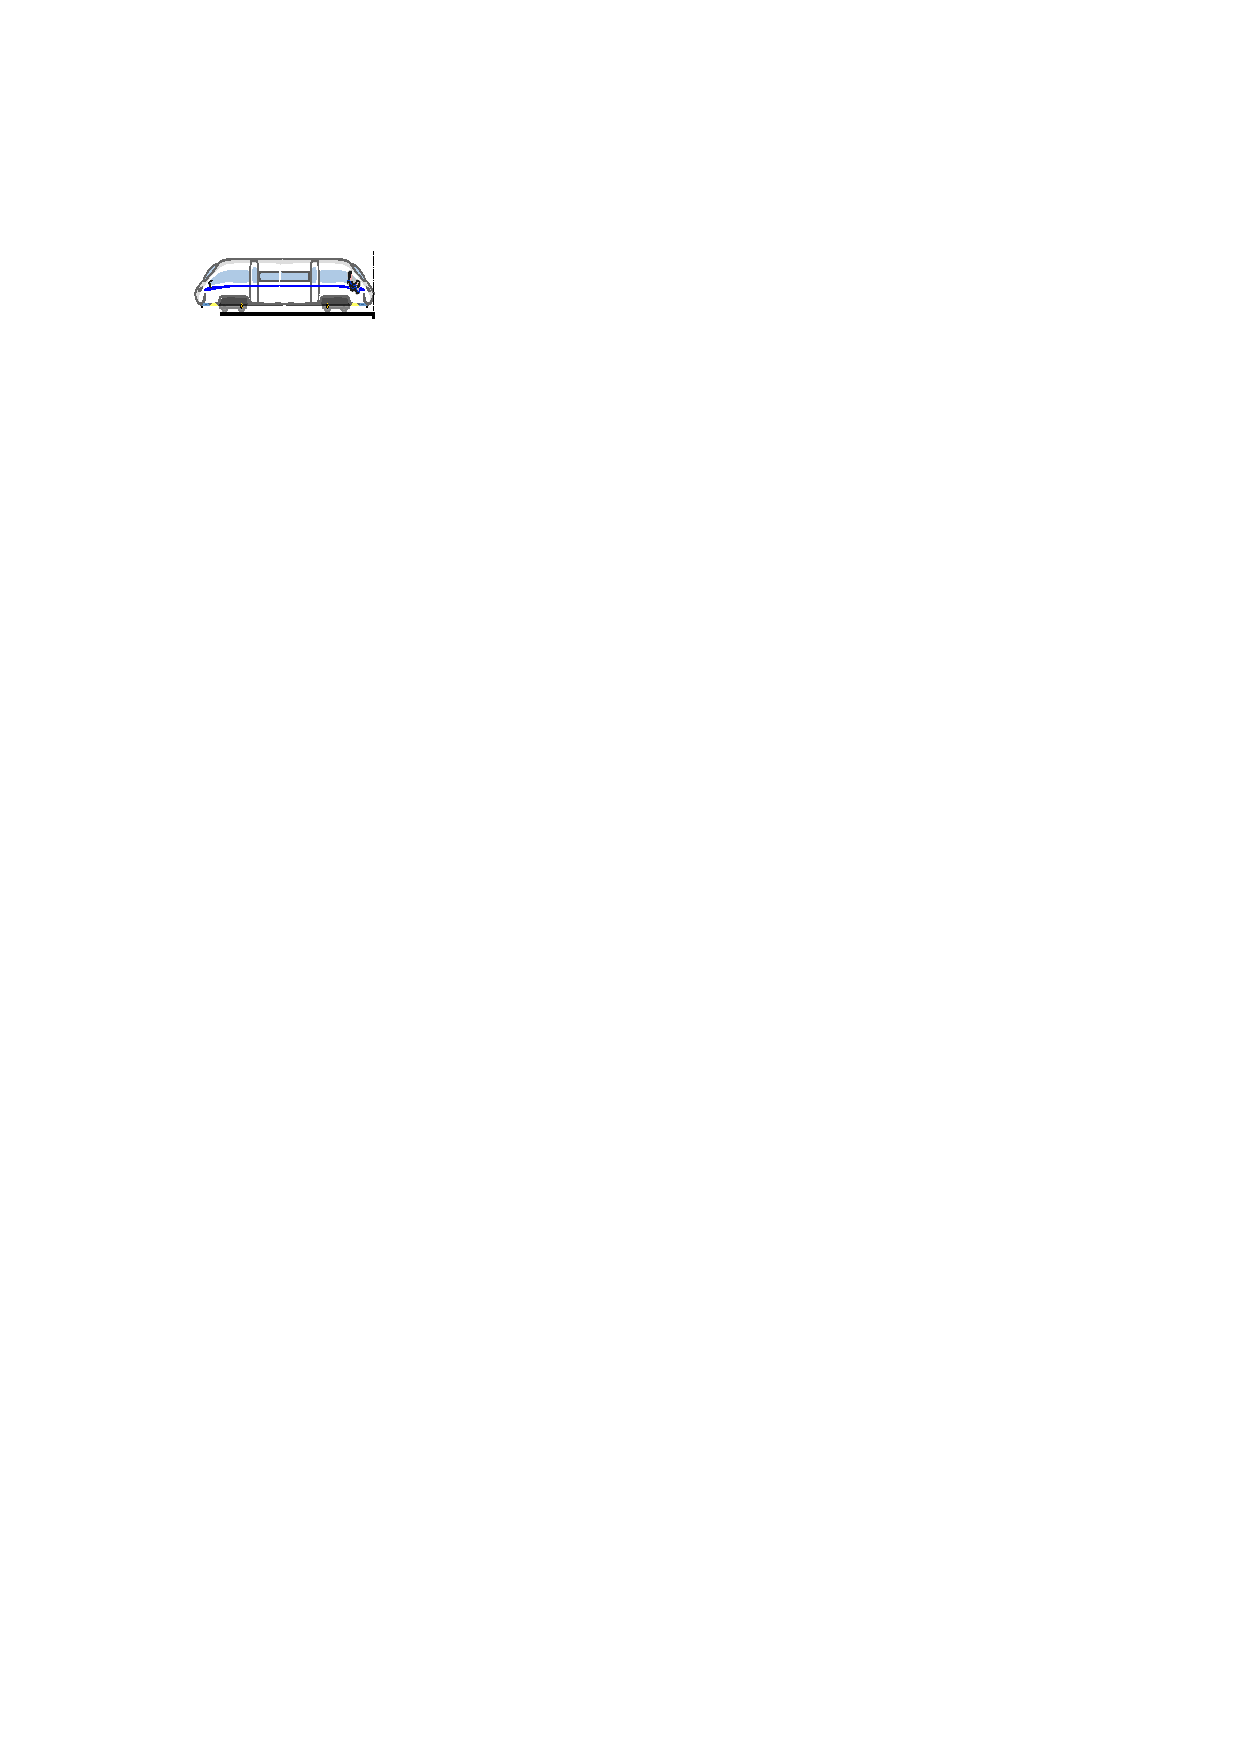
\includegraphics[scale=0.95]{figures/ch2/figure1.pdf}
	\caption{xxx示意图。 \\Fig~\ref{fig:ch2-f1}~Illustration of xxx.}
	\label{fig:ch2-f1}
\end{figure}

\vspace{-2em}

\begin{figure}[!htb]
	\centering
	\setlength{\belowcaptionskip}{-0.2cm} %调整图片caption与正文之间的间距,table用\abovecaptionskip。可自己调整。
	\addtocounter{subfigure}{-1}\subfigure[Subfig1.] {\subfigure[子图1] {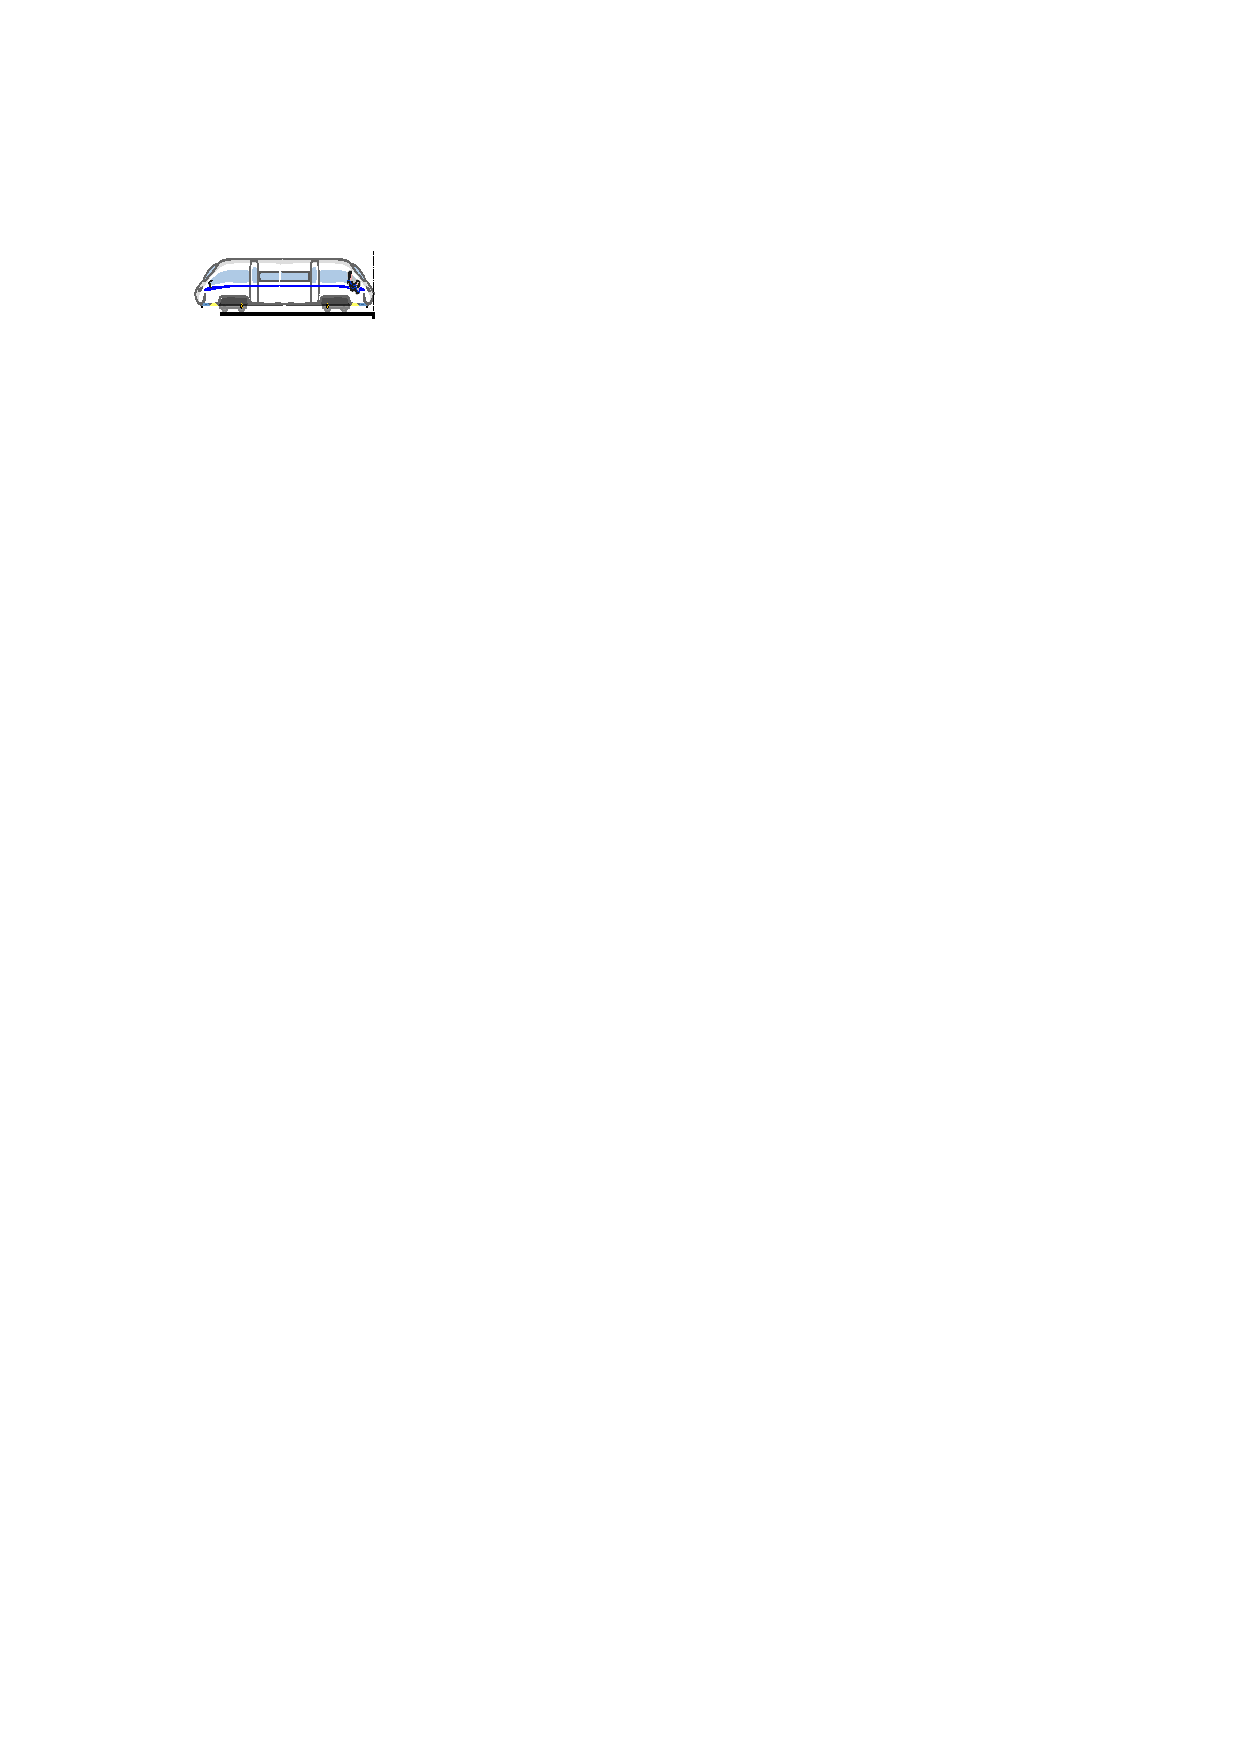
\includegraphics[scale=1]{figures/ch2/figure1.pdf}}}
	\hspace{20pt} %子图间距
	\addtocounter{subfigure}{-1}\subfigure[Subfig2.] {\subfigure[子图2]{ 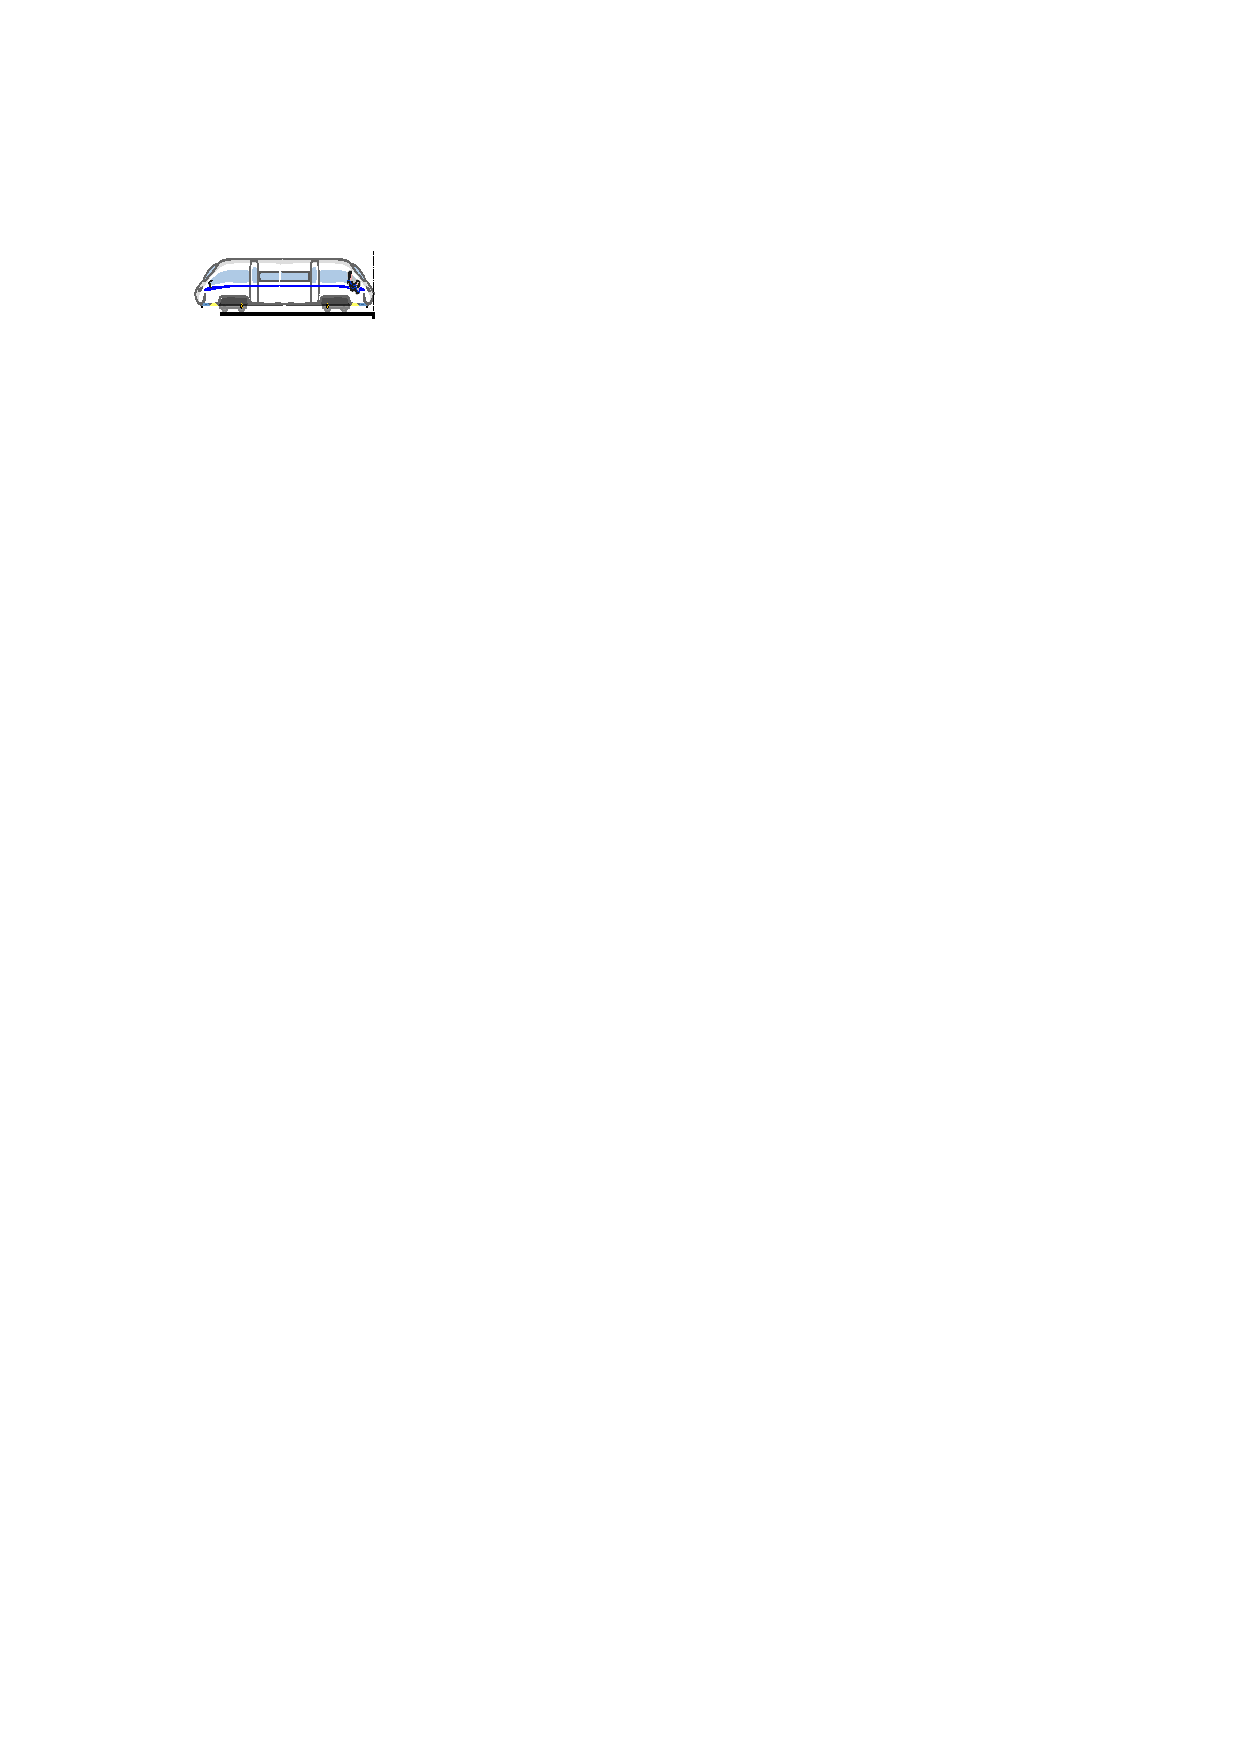
\includegraphics[scale=1]{figures/ch2/figure1.pdf}}}
	\caption{xxx示意图。\\Fig~\ref{fig:ch2-f2}~Illustration of xxx.}
	\label{fig:ch2-f2}
\end{figure} 


 								%第二章
	 \setlength{\baselineskip}{20pt}
\chapter{参考文献格式说明}
\label{cha:chap3}


\section{参考文献格式说明}

\textbf{命令:}\textbackslash cite\{xxx\},如深度学习\cite{lecunDeepLearning2015}。

\textbf{注意:}中文文献一定要在bib文件中添加语言标识language=\{zh\},否则作者名字无法正常以中文形式的‘等’进行省略,参考下面的例子\cite{zhou2021}:

@article\{zhou2021,
	
	\indent\indent title = \{图神经网络驱动的交通预测技术:探索与挑战\},
	
	\indent\indent author = \{周毅 and 胡姝婷 and 李伟 and 承楠 and 路宁 and 沈学民\},
	
	\indent\indent year = \{2021\},
	
	\indent\indent journal =\{物联网学报\},
	
	\indent\indent volume = \{5\},
	
	\indent\indent number = \{04\},
	
	\indent\indent pages = \{1--16\},
	
	\indent\indent issn = \{2096-3750\},
	
	\indent\indent \textbf{language=\{zh\}}
	
\}


\textbf{参考文献检查项}:论文完成后应仔细检查参考文献格式,下面总结了一些在论文审阅过程中常被指出的问题:

\begin{itemize}
	\item 参考文献格式参照下一小节
	\item 除Arxiv文章,所有文献必须有页码、年份,期刊论文还应有卷号、期号
	\item 检查同一会议/期刊的名称是否统一了
	\item 检查文献标题每个单词是否均首字母大写
	\item 检查发表会议/期刊名称每个单词是否均首字母大写
	\item 检查是否有重复文献
\end{itemize}








\subsection{参考文献格式}

参考文献是文中引用的有具体文字来源的文献集合。按照GB 7714《文后参考文献著录规则》的规定执行。参考文献的格式为:

著作:[序号]作者.译者.书名[M].版本(第一版不著录).出版地:出版社,出版时间:引用部分起止页.

期刊:[序号]作者.译者.文章题目[J].期刊名,年份,卷号(期数):引用部分起止页.

会议论文集:[序号]作者.译者.文章名[C]. //编者.论文集名,会议地址,会议时间.出版地:出版者,出版年.引用部分起止页.

学位论文:[序号]作者.题名[D].保存地点:保存单位,年份.引用部分起止页.

专利:[序号]专利申请者.专利文献题名[P].国别,专利文献种类,专利号.发布日期:引用部分起止页.

技术标准:[序号]起草责任者.标准代号.标准顺序号——发布年.标准名称.出版地.出版者.出版年份:引用部分起止页.

报纸: [序号]作者.题名[N].报纸名,出版日期(版次)


 								%第三章
	 \setlength{\baselineskip}{20pt}
\chapter{标题}
\label{cha:chap4}

\section{2级标题}
内容为小四号宋体


\subsection{3级标题}
内容为小四号宋体
 								%第四章
	 \setlength{\baselineskip}{20pt}
\chapter{标题}
\label{cha:chap5}

\section{2级标题}
内容为小四号宋体


\subsection{3级标题}
内容为小四号宋体
 								%第五章
	 \setlength{\baselineskip}{20pt}
\chapter{标题}
\label{cha:chap6}

\section{2级标题}
内容为小四号宋体


\subsection{3级标题}
内容为小四号宋体
 								%第六章
	 \setlength{\baselineskip}{20pt}
\chapter{总结与展望}
\label{cha:chap7}



\section{论文工作总结}

论文的结论是最终的、总体的结论,不是正文中各段的小结的简单重复。结论应该准确、完整、明确、精练。如果不可能导出应有的结论,也可以没有结论而进行必要的讨论。



\section{未来工作展望}

提出建议、研究设想、仪器设备改进意见以及尚待解决的问题等。 								%第七章


	%参考文献
	\bibliography{reference/ref}
	
	\backmatter %保持页面编号不变,取消后续章节编号

	%\begin{appendix}
	%	%%% Local Variables:
%%% mode: latex
%%% TeX-master: "../main"
%%% End:
\setlength{\baselineskip}{16pt}
\chapter{附录~A}

\begin{center}
\zihao{3}
\textbf{附录标题}
\end{center}

\indent
\zihao{5}
[内容为五号宋体。] 附录是作为论文主体的补充项目,并不是必须的。论文的附录依序用大写正体英文字母A、B、C……编序号,如:附录A。 %附录
	%\end{appendix}
	%%%% Local Variables:
%%% mode: latex
%%% TeX-master: "../main"
%%% End:

 \setlength{\baselineskip}{16pt}
%\chapter{索引}



\indent
\zihao{5}
%[内容为五号宋体。] 按照需要编排分类索引、著者索引、关键词索引等。        %索引
	\setlength{\baselineskip}{16pt}
\chapter{作者简历及攻读博士学位期间取得的研究成果}\zihao{5}
\setlength{\parindent}{0pt}

%[内容采用五号宋体]  包括教育经历、工作经历、攻读学位期间发表的论文和完成的工作等。行距16磅,段前后各为0磅。

\textbf{一、作者简历}
\vspace{10pt}


xxxxxxxx。



\vspace{10pt}
\textbf{二、发表论文}
\vspace{10pt}

\begin{enumerate}[leftmargin=*, parsep=5pt, label={[\arabic*]}]

	%非匿名
	\item \textbf{Author1}, Author2. Title. \emph{Journal/Conference}, Year, Volume(Issue), Pages. (SCI An分区, CCF 类别)
	
	%匿名
	\item \textbf{第一作者}. Title. \emph{Journal/Conference}, Year, Volume(Issue), Pages. (SCI An分区, CCF 类别)
	
\end{enumerate}



\vspace{10pt}
\textbf{三、参与科研项目}
\vspace{10pt}

\begin{enumerate}[leftmargin=*, parsep=5pt, label={[\arabic*]}]
	
	\item xxxxxx。
	
	\item xxxxxx。

\end{enumerate}



\vspace{10pt}
\textbf{四、获奖情况}
\vspace{10pt}

\begin{enumerate}[leftmargin=*, parsep=5pt, label={[\arabic*]}]
	
	\item xxxxxx。
	
	\item xxxxxx。
	
\end{enumerate}


      %作者简历
	%!TEX TS-program = xelatex
%!TEX encoding = UTF-8 Unicode

\setlength{\baselineskip}{16pt}
\chapter{答辩决议}\zihao{5}
\setlength{\parindent}{0pt}


\hspace{2em}[内容采用五号宋体]  行距16磅,段前后各为0磅。



\vspace{72pt}
\hspace{2em}答辩委员会主席签名:\hspace{1.5em}
\includegraphics[height=2.5\baselineskip]{signature.png}\hspace{4em}签字日期:xx 年 xx 月 xx 日

%\end{resolution}   %答辩决议
	 \setlength{\baselineskip}{16pt}
\chapter{独创性声明}\zihao{5}
%\thispagestyle{empty}




 
\hspace{2em}本人声明所呈交的学位论文是本人在导师指导下进行的研究工作和取得的研究成果,除了文中特别加以标注和致谢之处外,论文中不包含其他人已经发表或撰写过的研究成果,也不包含为获得北京交通大学或其他教育机构的学位或证书而使用过的材料。与我一同工作的同志对本研究所做的任何贡献均已在论文中作了明确的说明并表示了谢意。



\vspace{72pt}
 
\hspace{2em}学位论文作者签名:\hspace{1.5em}
\includegraphics[height=2.2\baselineskip]{signature.png}\hspace{4em}签字日期:xxx 年 xx 月 xx 日 

    %独创性声明
	
\chapter{学位论文数据集}\zihao{-4}


\setcounter{table}{0}
\renewcommand{\thetable}{1.\arabic{table}}

\begin{table}[!h]

\small 
\centering
\caption{数据集页}
\begin{tabular}{|p{2.6cm}|p{2.5cm}|p{2.6cm}|p{3.0cm}|p{2.3cm}|}
\hline

关键词$^*$  & 密级$^*$ & 中图分类号 & UDC & 论文资助 \\
\hline
xx &  公开 &  中图分类号查阅:http://www.ztflh.com/  &     &          \\  %对应上一行的标题对应填写: 关键词、密级、中图分类号、UDC、论文资助
\hline

\multicolumn{2}{|p{5.4cm}|}{学位授予单位名称$^*$} & 学位授予单位代码$^*$ & 学位类别$^*$ &  学位级别$^*$    \\
\hline
\multicolumn{2}{|p{5.4cm}|}{北京交通大学 }        &  10004               & 工学             &   博士     \\%对应上一行的标题对应填写: 学位类别、学位级别
\hline

\multicolumn{2}{|p{5.4cm}|}{论文题名$^*$} & \multicolumn{2}{p{5.4cm}|}{并列题名} &  论文语种$^*$    \\
\hline
\multicolumn{2}{|p{5.4cm}|}{ xxx }  & \multicolumn{2}{p{5.4cm}|}{ }        &   中文   \\ %对应上一行的标题对应填写: 论文题目、并列题名、论文语种
\hline

\ 作者姓名$^*$    &  \multicolumn{2}{p{5.4cm}|}{ xxx }   & 学号$^*$  &  xxx   \\%在对应空格上填写:作者姓名,学号 
\hline

\multicolumn{2}{|p{5.4cm}|}{ 培养单位名称$^*$ }  &  培养单位代码$^*$   & 培养单位地址  &  邮编   \\
\hline
\multicolumn{2}{|p{5.4cm}|}{ 北京交通大学 }  &  10004   & 北京市海淀区西直门外上园村3号  &  100044   \\
\hline

\multicolumn{2}{|p{5.4cm}|}{ 学科专业$^*$ }  &  研究方向$^*$   & 学制$^*$  & 学位授予年$^*$   \\
\hline
\multicolumn{2}{|p{5.4cm}|}{ 计算机科学与技术 }              &   数据与知识工程              &    xx年       &   xxx年   \\%对应上一行的标题对应填写:学科专业、 研究方向、学制、学位授予年

\hline
论文提交日期 $^*$    & \multicolumn{4}{l|}{ xx年xx月 }   \\%在对应空格上填写:论文提交日期 
\hline

\ 导师姓名$^*$    &  \multicolumn{2}{p{5.4cm}|}{ xxx }   & 职称$^*$  &  教授   \\%在对应空格上填写: 导师姓名、职称
\hline

\ 评阅人    &  \multicolumn{2}{p{5.4cm}|}{ 答辩委员会主席$^*$ }   & \multicolumn{2}{p{5.4cm}|}{ 答辩委员会成员 } \\
\hline
\ xxx,xxx,   &  \multicolumn{2}{p{5.4cm}|}{xxx}   & \multicolumn{2}{p{5.4cm}|}{xxx,xxx,xxx,xxx} \\%对应上一行的标题对应填写:评阅人、主席、成员
\ xxx,xxx,   &  \multicolumn{2}{p{5.4cm}|}{   }   & \multicolumn{2}{p{5.4cm}|}{   } \\
\ xxx          &  \multicolumn{2}{p{5.4cm}|}{   }   & \multicolumn{2}{p{5.4cm}|}{   } \\

\hline
\multicolumn{5}{|p{13.1cm}|}{ 电子版论文提交格式 \; 文本($\checkmark$)  图像( ) 视频( ) 音频( ) 多媒体( ) 其他( )}  \\
\multicolumn{5}{|p{13.1cm}|}{ 推荐格式:application/msword; application/pdf }  \\

\hline
\multicolumn{2}{|p{5.4cm}|}{ 电子版论文出版(发布)者  } & \multicolumn{2}{p{5.4cm}|}{电子版论文出版(发布)地  } & 权限声明\\
\hline
\multicolumn{2}{|p{5.4cm}|}{   } & \multicolumn{2}{p{5.4cm}|}{   } &  \\ %对应上一行的标题对应填写: 电子版论文出版(发布)者、发布地

\hline
论文总页数 $^*$    & \multicolumn{4}{l|}{ xxx }   \\%在对应空格上填写:页数
\hline
\multicolumn{5}{|p{13.1cm}|}{ 共33项,其中带$*$为必填数据,为22项。 }  \\



\hline 
\end{tabular}	
\end{table}





















 	    %数据集信息					


\end{document}




















